%% The following is a directive for TeXShop to indicate the main file
%%!TEX root = main.tex

% ===========================================================================================
\chapter{\textbf{Approach}}
\label{sec3:Approach}

In this chapter, the approach that we take towards designing and building a generic \ac{IDS} is discussed. The first part of the chapter describes in detail the work-flow undertaken by \ac{CORGIDS} along with the algorithm for intrusion detection. Next, it's followed by a motivating example which describes a use case where the physical invariants generated by \ac{CORGIDS} are able to detect intrusion.


\section{Work-flow of CORGIDS}
\ac{CORGIDS} is a generic intrusion detection system which exploits the correlation of the logical properties of the \ac{SUT} to detect intrusions. ~\autoref{fig:workflow} shows the key components and the work flow of \ac{CORGIDS}.

\begin{figure}[ht]
    \centering
    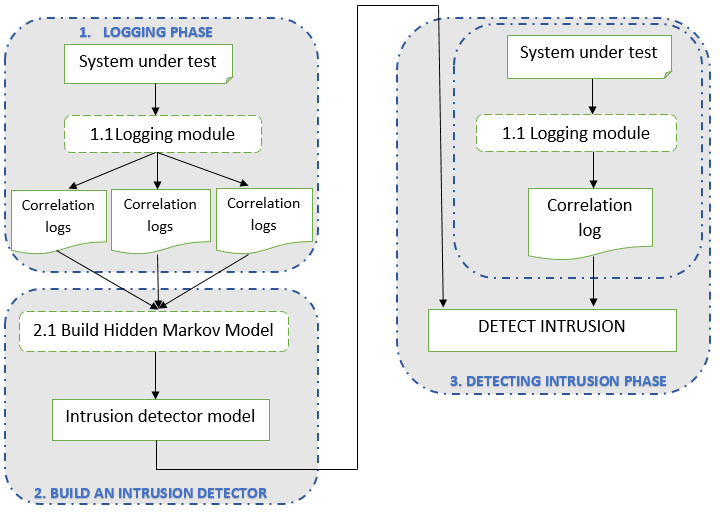
\includegraphics[scale=0.65,keepaspectratio = true]{Graphics/CORGIDSWorkflowNew.png}
    \caption{Workflow of CORGIDS}
    \label{fig:workflow}
\end{figure}

\ac{CORGIDS} workflow can be broken down into three main phases, namely, a) Logging Phase; b) Building an Intrusion Detector Phase; and c) Detecting Intrusion Phase. Each of the phases are explained below.

\begin{enumerate}
\item {Logging Phase}: The \textit{1. Logging Phase} in ~\autoref{fig:workflow} is the starting point for building an intrusion detector and for deploying it on a system for which intrusion detection is desired. \ac{SUT} is an input to this phase and is passed through the \textit{1.1 Logging module} in which it is manually instrumented to collect the values of the correlated properties\footnote{The approach of manually instrumenting the code to collect logs has been used by prior work~\cite{chen2018learning,aliabadi2017artinali}}. These properties are chosen by the user of the intrusion detection system based on the general knowledge of the \ac{SUT}. This phase will ensure that the traces which contain the values of the properties while the system is running are collected. Also, it is assumed that the source code of the \ac{SUT} is available and can be modified for instrumentation - this is reasonable as the developer of the system will deploy \ac{CORGIDS}. At the end of this \textit{logging phase}, the system traces containing the values of the logical properties of the \ac{SUT} are collected.

\item {Building an Intrusion Detector Phase}: In this phase, the system traces collected from the \textit{Logging Phase} are used to build an \ac{HMM} which behaviorally represents the \ac{SUT}. The pseudo code of the algorithm for building an intrusion detector is described below. To build an intrusion detector the system traces are fed into the \ac{HMM} model for its training in Line 1 in \textit{Procedure buildAnIntrusionDetector}.

\begin{algorithm}
  \caption{Building an intrusion detector}
  \textbf{Procedure buildAnIntrusionDetector (\textit{logs})}\;
  \nl \textit{trainedModel} = trainHMMModel (\textit{logs})\;
  \nl \ForEach{$l \in \textit{logs}$}{
    \textit{logLikelihood(i)} = log(\textit{trainedModel(l)})\;
    \textit{S} = sum of all \textit{logLikelihood(i)'s}\;
    }
  \nl \textit{M} = mean of \textit{S}\;
  \nl return \textit{trainedModel}, \textit{M}\;

  \textbf{Procedure trainHMMModel (\textit{logs})}\;
  \nl \ForEach{$\textit{hiddenStates} \in \{2, 3, \dots, J\}$}{
    \textbf{create an HMM model} \textit{model}(i)\;
    \textit{logLikelihood(i)} = log(\textit{model}(i))\;
    \nl \textbf{if} (\textit{logLikelihood}) \textless \textit{threshold} \textbf{then}\;
    \nl return \textit{model}(i)\;
  }
\end{algorithm}


Training of an \ac{HMM} is begun in \textit{procedure trainHMMModel} in Line 5, by varying the number of \textit{hiddenStates}. The number of hidden states is a free parameter of an \ac{HMM} which needs tuning in order to create a model which can be used for intrusion detection. Iteration begins with \ac{HMM} \textit{model(i)} with the starting value of two hidden states and is kept on increasing by one (Line 5). The log likelihood of the \textit{model(i)} is calculated which represents the goodness of the \textit{model(i)} fit of the model to the data that was used for constructing it.
The log likelihood is stored in variable \textit{logLikelihood(i)} as shown in Line 5. The \textit{threshold} in Line 6 represents the minimum difference between the current and previous \ac{HMM} log likelihood. Using threshold as a stopping criteria for \ac{HMM} has also been used in prior work~\cite{ferrer2000influence}. The best \ac{HMM} is returned in Line 7 with its parameters as the model to be used for intrusion detection. At this point the \textit{trainedHMMModel} is used to calculate the log likelihood for each of the training system traces (Line 2). As a by product, the mean of log likelihood is calculated (Line 2) to get the estimated log likelihood value \textit{M} (Line 3) for a training log. \textit{M} is then used for comparison in the later steps to detect intrusion. Creating \ac{HMM} by increasing the number of hidden states uses a significant amount of memory and computational power.
However as this phase needs to be carried out just once for a \ac{SUT}, it is not a major bottleneck. Once the intrusion detector \ac{HMM} is created, it can be used to detect an anomaly in the next phase. 

\item {Detecting Intrusion Phase}: This phase starts with the \textit{Logging Phase} which is used to collect the system trace from the \ac{SUT} while it is running. In this phase, only the system trace corresponding to the running \ac{SUT} is collected, rather than many different system traces. 
The trace generated is then used together with the intrusion detector built in the \textit{Building an Intrusion Detector Phase}. Using the \ac{HMM} model and its saved parameters, the log likelihood of the current system trace is calculated and compared with the mean log likelihood \textit{M} calculated in the \textit{Building an Intrusion Detector} in Line 6. If the log likelihood of the system trace is less than a specified range ($\delta$) from \textit{M}, it signifies that the system trace does not follow the behavior which was observed when the \ac{HMM} was being trained. 
The specified range ($\delta$) is found by running a sensitivity analysis (Section \ref{sensitivityAnalysis}). Further, as the system traces used for building the \ac{HMM} were assumed to be correct (i.e., not attacked), this implies that the current system trace represents a system under attack.  
Thus, current state of the \ac{SUT} is flagged to be malicious. 
\end{enumerate}


\section{A motivating example}

\begin{figure}[ht]
    \centering
    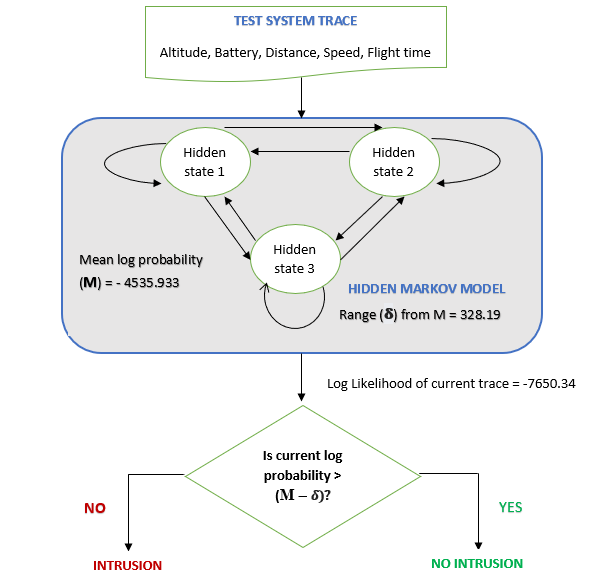
\includegraphics[scale=0.75,keepaspectratio = true]{Graphics/CORGIDSApproach.png}
    \caption{Approach of CORGIDS}
    \label{fig:approach}
\end{figure}

The earlier example of an \ac{UAV} from ~\autoref{ch:Introduction} is used in this chapter to illustrate how \ac{CORGIDS} can be used to detect intrusions in ~\autoref{fig:approach}. As described in ~\autoref{ch:Introduction}, an \ac{UAV} has physical properties such as the current altitude, battery percentage left, distance traveled, current speed and flight time. These physical properties are correlated to each other as per the laws of physics. The approach which will be used to detect an intrusion in an \ac{UAV} is elaborated, using the work-flow described in ~\autoref{fig:approach}. Distance spoofing attack scenario of the \ac{UAV} is used as an example. This attack is explained in detail in ~\autoref{ch:Attacks}.

First the \textit{Logging Phase} starts, where the \ac{UAV} is instrumented to collect the correlated properties such as altitude, battery percentage left, distance traveled, speed and flight time. The above properties are collected at regular intervals of time to form the system traces. A section of the sample system trace collected is shown in Table~\ref{tab:nonFaultyCorrelationLog}. In the trace, it can be observed that all the properties are correlated  with each other, and that the correlations are fairly stable. For instance, if the \textit{Speed} of the \ac{UAV} increases, the \textit{Distance traveled} will also increase proportionally. Further, the \textit{Distance traveled} property can have values that are either increasing or stagnant. Multiple iterations of the \ac{UAV} were run by varying the routes it travels, to collect non-faulty system traces from it.

\begin{table}
\centering
  \caption{Slice of a non-faulty system trace obtained while flying an UAV on a random route}
  \label{tab:nonFaultyCorrelationLog}
  \scalebox{0.9}{
  \begin{tabular}{|p{1.2cm}|p{1.2cm}|p{1.85cm}|p{0.9cm}|p{1.7cm}|}
 \toprule
\textbf{Altitude (m)}&\textbf{Battery left (\%)}&\textbf{Distance traveled (m)}&\textbf{Speed (m/s)}&\textbf{Flight time (s)}\\
  \hline
..&..&..&..&..\\
40&89&42.1445&1&38.32\\
40&89&44.2563&2&39.342\\
40	&89	&47.2397	&3	&40.356\\
40	&89	&51.0202	&3	&41.376\\
40	&88	&55.2434	&4	&42.345\\
40	&88	&59.5897	&4	&43.346\\
40	&88	&64.1632	&4	&44.335\\
41	&88	&68.8979	&4	&45.323\\
41	&88	&73.7389	&4	&46.351\\
41	&87	&78.6564	&4	&47.448\\
41	&87	&83.6196	&4	&48.551\\
41	&87	&88.6138	&4	&49.61\\
41	&87	&93.627	    &5	&50.604\\
41	&86	&98.6659	&5	&51.507\\
..&..&..&..&..\\
\hline
\end{tabular}
}
\end{table}

\begin{table}
\centering
\caption{Slice of a faulty system trace obtained while an UAV was flying on a random route and infected by distance spoofing attack}
\label{tab:faultyCorrelationLog}
\scalebox{0.9}{
\begin{tabular}{|p{1.2cm}|p{1.2cm}|p{1.85cm}|p{0.9cm}|p{1.7cm}|}
\toprule   \textbf{Altitude (m)}&\textbf{Battery left (\%)}&\textbf{Distance traveled (m)}&\textbf{Speed (m/s)}&\textbf{Flight time (s)}\\
  \hline
..&..&..&..&..\\
 40 & 89 & 42.7868 & 1 & 38.206 \\
 40 & 89 & 45.2942 & 2 & 39.279\\
 41 & 89 & 48.6934 & 3 & 40.272\\
 42 & 89 & 42 &	4 &	41.261\\
42&	88&	57.0199&	4&	42.267\\
43&	88&	46&	4&	43.285\\
43&	88&	66.0254&	4&	44.357\\
44&	88&	70.7879&	4&	45.347\\
44&	87&	65&	4&	46.292\\
45&	87&	80.5709&	4&	47.37\\
46&	87&	85.5441&	4&	48.386\\
46&	87&	49&	4&	49.373\\
47&	86&	54&	4&	50.367\\
47&	86&	100.6006& 4&	51.402\\
..&..&..&..&..\\
\hline
\end{tabular}
}
\end{table}
In the second phase, \textit{Build an Intrusion Detector}, the system traces collected from \textit{Logging Phase} are used. \ac{HMM} are generated, \textit{model(i)}, by varying the number of hidden states in line 5 in the given algorithm. Then for each of the \textit{model(i)} generated, the \textit{logLikelihood(i)} is calculated in line 5 to determine if the \textit{model(i)} fits the data used for constructing it. To accomplish this, the difference in \textit{logLikelihood(i)} is compared to the \textit{threshold} in line 6 and if the \textit{threshold} is met, \textit{model(i)} is returned in line 7. It was found that an \ac{HMM} with 15 hidden states is the one which met the threshold. As showing 15 hidden states in the ~\autoref{fig:approach} will clutter it, we simplified the model by showing only 3 hidden states. Further, in lines 2 and 3, the sum of \textit{logLikelihood's} for all the correlated logs \textit{S} is calculated from which \textit{M} (mean log likelihood) = $-4535.933$ is extracted.

To demonstrate how an attack will be detected by \ac{CORGIDS}, we consider an attack where the attacker decides to spoof the values of distance traveled found inside the data packets being transferred from the \ac{UAV} to the \ac{GCS}. An \ac{UAV} periodically send the flight data to the \ac{GCS} to keep it updated about its whereabouts. To intervene the working of \ac{UAV}, the attacker gains access to the communication channel between the \ac{UAV} and \ac{GCS}. Now, an attacker can easily change the contents of the data packets being transferred.

In the final phase, when the \ac{UAV} is deployed in production, the \textit{Detecting Intrusion Phase} is active in the \ac{GCS} and uses the current system trace produced from the logging module along with the trained HMM to detect intrusion. A slice of the faulty-system trace is shown in Table~\ref{tab:faultyCorrelationLog}. As can be observed, the values of distance traveled are changing but do not follow the correlations observed in the earlier trace in Table~\ref{tab:nonFaultyCorrelationLog}. As only the distance traveled values have been tampered with, leaving other logical properties intact, we get a correlation which is different from the one that is expected by the trained \ac{HMM}. This results in the difference between the mean and current log likelihood values being greater than the threshold value - say ($\delta$). From ~\autoref{fig:approach}, the log likelihood of the current system trace is more than $\delta$ from the \textit{M} (mean log likelihood). Therefore, \ac{CORGIDS} flags the current state of the \ac{UAV} to be \textit{malicious}. The value of the threshold used in this example, ($\delta$) = $328.19$ is determined experimentally in section \ref{sensitivityAnalysis}. 

\section{Summary}
In this chapter we introduced \ac{CORGIDS} by first describing its workflow, phase by phase. As discussed in the chapter, \ac{CORGIDS} deduces the behavior of the \ac{SUT} in the \textit{Build an intrusion detector phase}. This behavior is then used later in the \textit{Intrusion detection phase} to flag any malicious activities. \ac{CORGIDS} is novel and different from other prior work discussed in previous chapter because it dynamically generates the physical invariants for the \ac{CPS} and to do it uses \ac{HMM}. \ac{HMM} can exceptional in inferring the correlation/likelihood between different variables. Also, in the first section of the chapter we demonstrate with the help of an algorithm how a trained \ac{HMM} is generated with variables such as number of training traces and threshold. Later, we provide an example which walks through the 3 phases of work-flow of \ac{CORGIDS} along with the possible attack scenario. The example explained is taken from our experiments and contains the real values of mean log likelihood, acceptable range of the trained intrusion detection model. The decision making process of \ac{CORGIDS} is shown pictorially to enhance understanding.

\endinput
=====================================================================
